\documentclass[11pt,a4paper]{article}

\usepackage[utf8]{inputenc}
\usepackage[T1]{fontenc}
\usepackage{lmodern}
\usepackage[margin=2.6cm]{geometry}
\usepackage{amsmath,amssymb}
\usepackage{graphicx}
\usepackage{booktabs}
\usepackage{caption}
\usepackage{subcaption}
\usepackage{authblk}
\usepackage[hidelinks]{hyperref}
\usepackage{natbib}
\usepackage{microtype}

\captionsetup{font=small,labelfont=bf}

\newcommand{\Rec}{\mathrm{Re}_c}
\newcommand{\Ret}{\mathrm{Re}_\tau}
\newcommand{\Reth}{\mathrm{Re}_\theta}
\newcommand{\bbar}{\bar{\beta}}
\newcommand{\dnn}{\delta_{99}}

\title{\bfseries Separating pressure-gradient history from Reynolds-number
effects in turbulent wing boundary layers}

\author[1]{\textit{Author Name}}
\affil[1]{\textit{Affiliation}}
\date{\today}

\begin{document}
\maketitle

\begin{abstract}
\noindent
Turbulent boundary layers on wings are shaped both by the local pressure
gradient and by the pressure gradient they have already passed through, and
separating those from Reynolds-number effects requires holding one fixed
while varying the other. The NACA4412 section is a natural vehicle, because
its pressure distribution is almost independent of Reynolds number, and
\citet{vinuesa2018} used exactly this to attribute the differences between
four large-eddy simulations at $\Rec = 10^5$ to $10^6$ to Reynolds number
alone. We revisit that database and show, first, that the matched-$\beta$
premise holds only to tens of percent: the Clauser parameter decreases
monotonically with Reynolds number at every station, running on average
$42\%$ higher at $\Rec = 2\times10^5$ than at $10^6$ over
$0.25 \le x/c \le 0.95$. Because every quantity of interest increases with
$\beta$, the residual mismatch acts in the same direction as the effect
being measured. We then fit a three-term power law in which the local
pressure gradient, a kernel-weighted memory of the upstream pressure
gradient, and the friction Reynolds number appear as separate factors, with
the memory length fitted inside each training fold. The law predicts a
held-out Reynolds number to $1.2$--$9.2\%$ and, being linear in logarithms,
splits the difference between two cases exactly. For the outer-region
Reynolds stresses---the quantities that carry the original argument---
$64$--$77\%$ of the apparent Reynolds-number trend is attributable to the
residual $\beta$ mismatch; for the wall and integral quantities and for
turbulent kinetic energy production, Reynolds number dominates and the
original reading stands. The law transfers unchanged from the NACA4412 at
$5^\circ$ to a NACA0012 at $0^\circ$ with $2.5$--$9.8\%$ median error on
five of six quantities. Finally, an exhaustive search over expressions
selects the interaction between local $\beta$ and the memory ratio for all
six targets, indicating that history and local pressure gradient multiply
rather than acting as separable factors.
\end{abstract}

\section{Introduction}

Turbulent boundary layers (TBLs) subjected to streamwise pressure gradients
(PGs) occur wherever a surface is curved, and the adverse-pressure-gradient
(APG) layer on the suction side of a wing is among the most consequential
cases. Its behaviour is not set by the local pressure gradient alone.
\citet{clauser1956} observed that the outer part of a boundary layer has a
long memory, so that its state depends on the sequence of conditions it has
passed through, and \citet{bobke2017} demonstrated that two layers at the
same local Clauser parameter
\begin{equation}
  \beta = \frac{\delta^*}{\tau_w}\frac{\mathrm{d}P_e}{\mathrm{d}x}
  \label{eq:beta}
\end{equation}
can differ substantially if they arrived there by different routes.

Disentangling history from Reynolds number requires a configuration in
which one can be held fixed. The NACA4412 section provides it: at moderate
angles of attack its pressure distribution is nearly independent of
Reynolds number \citep{pinkerton1938}, so simulations at different $\Rec$
nominally experience the same $\beta(x)$. \citet{vinuesa2018} exploited
this with four well-resolved large-eddy simulations (LES) spanning
$\Rec = 10^5$ to $10^6$ at $5^\circ$ incidence, comparing each against a
zero-pressure-gradient (ZPG) layer at matched $\Ret$. They reported that
the ratios of edge velocity, shape factor, Reynolds stresses and outer-layer
production all decrease with $\Rec$, and concluded that lower-Reynolds-number
layers are more sensitive to a given pressure gradient, with two
complementary mechanisms---one tied to Reynolds number, one to the APG---
energising the outer region.

That conclusion rests entirely on $\beta(x)$ being matched between the
cases. In Section~\ref{sec:confound} we show that it is matched only to
tens of percent, and that the residual varies monotonically with Reynolds
number, so that it is confounded with the quantity being measured. The rest
of the paper supplies the decomposition that the original comparison could
not: a model in which local pressure gradient, flow history and Reynolds
number enter as separate, identifiable terms.

Our contributions are:
\begin{enumerate}
  \item a reproduction of \citet{vinuesa2018} from the distributed database,
        agreeing to a median of $0.75\%$ across 48 published quantities, with
        two documented discrepancies in how the database must be read
        (Section~\ref{sec:data});
  \item a quantification of the residual $\beta$ mismatch and its direction
        (Section~\ref{sec:confound});
  \item a three-term power law with a fitted memory length that predicts a
        held-out Reynolds number to $1.2$--$9.2\%$ and splits the difference
        between cases exactly (Sections~\ref{sec:model}--\ref{sec:decomp});
  \item cross-geometry validation on a NACA0012, and an exhaustive symbolic
        search showing that history and local pressure gradient multiply
        (Section~\ref{sec:general}).
\end{enumerate}

\section{Database and reproduction}
\label{sec:data}

We use the publicly documented WING database of \citet{vinuesa2018} and
\citet{tanarro2020}: well-resolved LES of the flow around a NACA4412 at
$\Rec = 10^5$, $2\times10^5$, $4\times10^5$ and $10^6$ at $5^\circ$
incidence, computed with the spectral-element code Nek5000, plus a NACA0012
at $\Rec = 4\times10^5$. Statistics are distributed at 50 chordwise
stations per side, in the local tangential and wall-normal frame, with
$U_e$ and $\dnn$ obtained by the diagnostic-scaling method of
\citet{vinuesa2016}. We follow the original analysis window
$0.25 \le x/c \le 0.95$: below it the layer is still accelerating and close
to the trip at $x/c = 0.1$; above it the structures detach from the wall and
the boundary-layer description loses meaning.

\paragraph{Reproduction.} Interpolating to the exact stations quoted in the
source, all 48 tabulated quantities (Tables 3 and 4 and the maxima quoted in
its Section 3.1) are recovered to a median absolute error of $0.75\%$, with
$47$ of $48$ within $5\%$; the residual is dominated by $\beta$ being
published to two significant figures.

\paragraph{Two caveats in reading the files.} Both are easy to get wrong and
neither is stated in the distribution. First, the velocity scale behind every
shipped integral quantity---$C_f$, $\mathrm{Re}_{\delta^*}$, $\Reth$,
$\delta^*$ and $\theta$---is the \emph{maximum} tangential velocity of each
profile, not the \texttt{Ue} field stored alongside it. We verified this by
inverting each quantity for the velocity it implies, obtaining agreement with
$\max(U)$ to machine precision across all nine distributed cases. Using
\texttt{Ue} instead, the obvious reading, puts the integral thicknesses out by
$9$--$13\%$ and $C_f$ by about $6\%$. Second, $\beta$ cannot be recomputed
from the 50 stored stations to better than a median of $\sim\!7\%$, because
they under-resolve $\mathrm{d}P_e/\mathrm{d}x$; near the leading edge the
recomputed value disagrees in sign. We therefore use the distributed $\beta$
throughout.

\section{The matched-$\beta$ premise}
\label{sec:confound}

\begin{figure}[t]
  \centering
  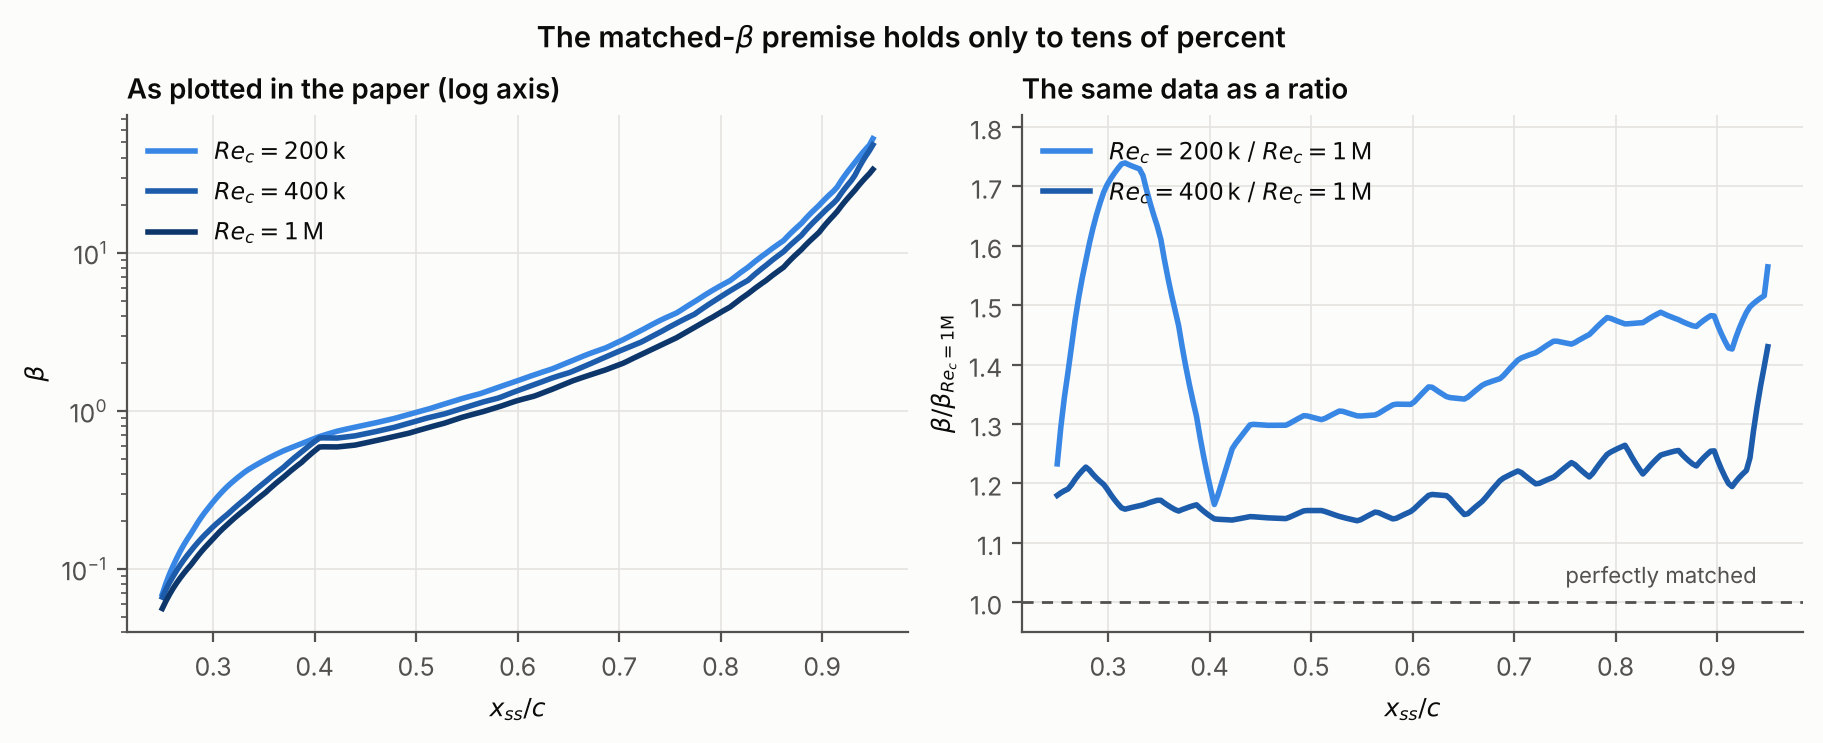
\includegraphics[width=\textwidth]{figures/fig_beta_confound.png}
  \caption{The Clauser parameter on the suction side for the three
  higher-Reynolds-number cases. \textbf{Left:} as conventionally plotted, on
  a four-decade logarithmic axis, on which the curves appear to collapse.
  \textbf{Right:} the same three curves as a ratio to the $\Rec = 10^6$
  case. The mismatch is $20$--$50\%$ and monotone in Reynolds number.}
  \label{fig:confound}
\end{figure}

\citet{vinuesa2018} describe the $\Rec \ge 2\times10^5$ cases as subjected
to ``approximately the same'' $\beta(x)$, with relative differences ``on the
order of 10\%'' arising only beyond $x/c > 0.9$. Over the analysis window
the distributed data give
\begin{equation*}
  \frac{\beta(\Rec = 2\times10^5)}{\beta(\Rec = 10^6)} = 1.42
  \;(1.17\text{--}1.74), \qquad
  \frac{\beta(\Rec = 4\times10^5)}{\beta(\Rec = 10^6)} = 1.19
  \;(1.14\text{--}1.43),
\end{equation*}
with $\beta$ decreasing monotonically with Reynolds number at \emph{every}
station. The source's own Table 4 is consistent: at $x/c = 0.7$ it lists
$\beta = 2.6$, $2.4$ and $2.0$, a ratio of $1.30$ rather than $1.10$. The
apparent collapse in its Figure 5 is a consequence of the logarithmic axis,
on which a factor of $1.4$ is a hairline offset (Figure~\ref{fig:confound}).

This matters because the reported effect and the residual mismatch act in
the same direction. The ratios $\Phi$ of wing to ZPG quantities all increase
with $\beta$; $\beta$ decreases with $\Rec$; therefore $\Phi$ would decrease
with $\Rec$ even if the boundary layer had no intrinsic Reynolds-number
sensitivity at all. Nothing here contradicts the physical mechanism
proposed in the original work, which is independently supported by the
wall-normal velocity distributions. What is missing is the attribution.

\section{A power law with a fitted memory}
\label{sec:model}

\subsection{History variable}

We summarise the upstream pressure gradient by an exponentially weighted
mean,
\begin{equation}
  \bbar(x;\ell) =
  \frac{\displaystyle\int_{x_0}^{x} \beta(\xi)\,
        \exp\!\left(-\frac{s(x)-s(\xi)}{\ell}\right)\mathrm{d}\xi}
       {\displaystyle\int_{x_0}^{x}
        \exp\!\left(-\frac{s(x)-s(\xi)}{\ell}\right)\mathrm{d}\xi},
  \qquad \ell = m\,\dnn(x),
  \label{eq:kernel}
\end{equation}
where $s$ is arc length along the surface and the memory length scales with
the local boundary-layer thickness, so that the kernel widens as the layer
grows. Normalising by the kernel's own integral over the available upstream
distance is essential: without it, stations near the start of the data would
be assigned a small history merely because less wing lies upstream, and the
model would learn chordwise position rather than memory. As defined,
$\bbar$ is a weighted mean of $\beta$ and is directly comparable with the
local value. Integration always uses arc length rather than $x/c$, since the
surface slope departs far from unity on the forward part of the section.

\subsection{Functional form}

We fit, for each target $y$,
\begin{equation}
  y = C\,\beta^{a_1}\,
      \left(\frac{\bbar}{\beta}\right)^{a_2}\,
      \Ret^{\,a_3}.
  \label{eq:law}
\end{equation}
Three considerations fix this form. It is the smallest expression with a
separate term for each candidate cause. It is linear in logarithms, so
Shapley attribution is exact and analytic rather than sampled, and the
difference between two cases decomposes without approximation. And with
roughly 40 usable stations per Reynolds number, three coefficients and one
length is close to the most the data supports---consistent with our finding
that ridge regression in log space outperforms gradient boosting on every
target under leave-one-Reynolds-number-out validation, because the held-out
fold requires extrapolating in $\Ret$ rather than interpolating.

The history term is deliberately the \emph{ratio} $\bbar/\beta$ rather than
$\bbar$. Parameterised as separate powers of $\beta$ and $\bbar$, the two are
nearly collinear---at short memory $\bbar \to \beta$---and the fit returns
equal-and-opposite exponents of order $\pm 7$ that are unstable and
uninterpretable. Since
$\beta^{a_1}\bbar^{a_2} = \beta^{a_1+a_2}(\bbar/\beta)^{a_2}$, the ratio
form is an exact reparameterisation of the same model class in which the two
terms carry distinct meanings, and in which the history term switches itself
off as $\ell \to 0$.

\subsection{Fitting and validation}

For fixed $\ell$ the model is linear and solved exactly by regularised least
squares, leaving a one-dimensional search over $\ell$ (variable projection).
This is global over the searched interval and has no learning rate,
initialisation or stopping rule.

Validation is leave-one-Reynolds-number-out: the model must predict a
Reynolds number it has never seen. Random splits would be meaningless, since
adjacent stations on the same wing are nearly the same boundary layer.
Crucially, $\ell$ is selected by an inner leave-one-case-out \emph{within}
the training fold; selecting it on held-out error, as a naive scan does, is
selection on the test set. The $\Rec = 10^5$ case is excluded throughout: the
original work shows it is not a well-behaved TBL, and its final station has
separated.

\subsection{Identifiability}

On synthetic data generated from Equation~\eqref{eq:law} the fitter recovers
$\ell$ and all three exponents to four significant figures. Adding $0.2\%$
noise in log space---well below the scatter in the LES statistics---moves the
fitted $\ell$ by $15$--$27\%$ and $a_2$ by up to $65\%$, because a shorter
memory shrinks $\log(\bbar/\beta)$ and a larger $|a_2|$ compensates almost
exactly. We therefore quote $\ell$ to a factor of order $1.3$ and never to two
digits. The decomposition of Section~\ref{sec:decomp} is built from the
product $a_2\log(\bbar/\beta)$, in which the trade-off cancels; we verify
below that forcing $\ell$ to half or double its fitted value leaves the
result essentially unchanged.

\section{Decomposition}
\label{sec:decomp}

\begin{table}[t]
  \centering
  \small
  \caption{Fitted law under leave-one-Reynolds-number-out, with the memory
  length refitted inside each training fold. $\ell$ is in multiples of the
  local $\dnn$; the range is across folds. Outer-region quantities are
  sampled at $y_n/\dnn = 0.2$.}
  \label{tab:fit}
  \begin{tabular}{lcccccc}
    \toprule
    target & $\ell/\dnn$ & (fold range) & $a_1$ & $a_2$ & $a_3$ &
    held-out error \\
    \midrule
    $H$                      & 0.59 & 0.57--0.70 & $ 0.03$ & $ -0.88$ & $-0.07$ & 1.15\% \\
    $C_f$                    & 0.43 & 0.41--0.48 & $-0.04$ & $  8.14$ & $-0.35$ & 2.36\% \\
    $U_e^+$                  & 0.43 & 0.41--0.48 & $ 0.02$ & $ -4.07$ & $ 0.17$ & 1.20\% \\
    $\overline{u_t^2}^+$     & 0.46 & 0.46--0.60 & $ 0.09$ & $ -7.45$ & $-0.14$ & 9.24\% \\
    $\overline{u_tv_n}^+$    & 0.45 & 0.41--0.52 & $ 0.15$ & $ -6.67$ & $ 0.06$ & 3.82\% \\
    $P_k^+$                  & 0.47 & 0.46--0.58 & $ 0.17$ & $-11.36$ & $-0.97$ & 6.08\% \\
    \bottomrule
  \end{tabular}
\end{table}

Table~\ref{tab:fit} reports the fit. The memory length is short and stable
across folds for every quantity, $\ell \approx 0.4$--$0.6\,\dnn$, and the
inner objective is sharply peaked: error rises by a factor of $10$--$24$ as
$\ell \to 0$, where the history term switches off, and by $5$--$10$ by
$\ell = 17\,\dnn$. Flow history carries a great deal of information, over a
distance of order the local boundary-layer thickness.

Because Equation~\eqref{eq:law} is linear in logarithms, the difference
between two cases at matched chordwise position splits exactly:
\begin{equation}
  \underbrace{\Delta \log y}_{\text{observed}} =
  \underbrace{a_1\,\Delta\log\beta
            + a_2\,\Delta\log(\bbar/\beta)}_{\text{pressure gradient}}
  + \underbrace{a_3\,\Delta\log\Ret}_{\text{Reynolds number}} .
  \label{eq:split}
\end{equation}

\begin{figure}[t]
  \centering
  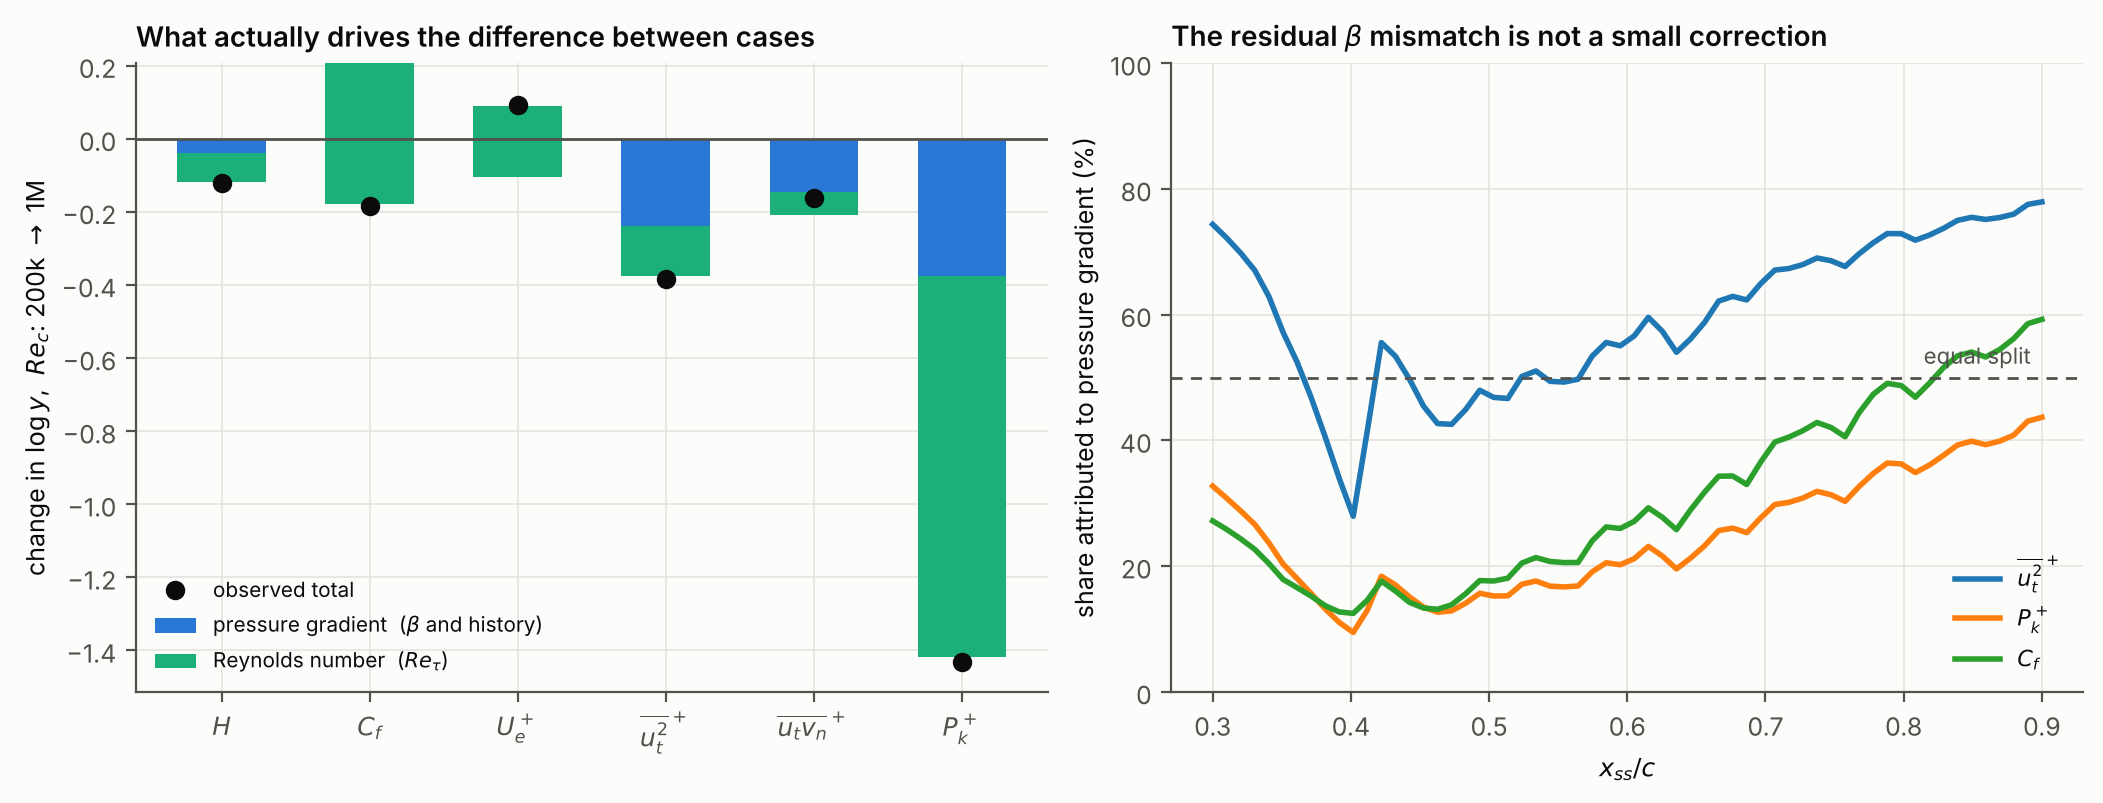
\includegraphics[width=\textwidth]{figures/fig_decomposition.png}
  \caption{\textbf{Left:} the change from $\Rec = 2\times10^5$ to $10^6$,
  averaged over $0.30 \le x/c \le 0.90$, split by
  Equation~\eqref{eq:split}. The split is exactly additive, so the stack
  reaches the observed total. \textbf{Right:} the share attributed to the
  pressure gradient as a function of chordwise position.}
  \label{fig:decomp}
\end{figure}

Figure~\ref{fig:decomp} and Table~\ref{tab:split} give the result. For the
outer-region Reynolds stresses, the majority of the apparent
Reynolds-number trend is attributable to the residual $\beta$ mismatch:
$64\%$ for $\overline{u_t^2}^+$ and $77\%$ for $\overline{u_tv_n}^+$. These
are precisely the quantities on which the original argument leans most
heavily. For the wall and integral quantities, and for TKE production,
Reynolds number dominates at $65$--$73\%$ and the original reading stands.

\begin{table}[t]
  \centering
  \small
  \caption{Share of the $\Rec = 2\times10^5 \to 10^6$ change attributable to
  each cause, with robustness checks. Columns 3--5 repeat the
  pressure-gradient share for a different pair of cases and for the memory
  length forced off its fitted value.}
  \label{tab:split}
  \begin{tabular}{lcc ccc}
    \toprule
    & \multicolumn{2}{c}{attributed share} &
      \multicolumn{3}{c}{PG share under perturbation} \\
    \cmidrule(lr){2-3}\cmidrule(lr){4-6}
    target & pressure gradient & Reynolds &
    $4\!\times\!10^5\!\to\!10^6$ & $\ell\times0.5$ & $\ell\times2$ \\
    \midrule
    $\overline{u_tv_n}^+$ & \textbf{77\%} & 23\%          & 73.5\% & 83.7\% & 80.2\% \\
    $\overline{u_t^2}^+$  & \textbf{64\%} & 36\%          & 60.4\% & 61.1\% & 59.3\% \\
    $U_e^+$               & 35\%          & \textbf{65\%} & 31.1\% & 33.3\% & 36.1\% \\
    $C_f$                 & 35\%          & \textbf{65\%} & 31.1\% & 33.3\% & 36.1\% \\
    $H$                   & 34\%          & \textbf{66\%} & 31.2\% & 34.3\% & 33.4\% \\
    $P_k^+$               & 27\%          & \textbf{73\%} & 23.7\% & 24.7\% & 25.5\% \\
    \bottomrule
  \end{tabular}
\end{table}

The split survives three checks. Changing the compared pair from
$2\times10^5 \to 10^6$ to $4\times10^5 \to 10^6$ moves the shares by at most
$3$ percentage points. Forcing $\ell$ to half or double its fitted value
moves them by at most $7$ points, usually $1$--$3$, confirming that the
$\ell$--$a_2$ trade-off cancels in the product. And the fitted law reproduces
the observed change to within $2$--$10\%$ (Figure~\ref{fig:decomp}, left).

\section{Generalisation and functional form}
\label{sec:general}

\begin{figure}[t]
  \centering
  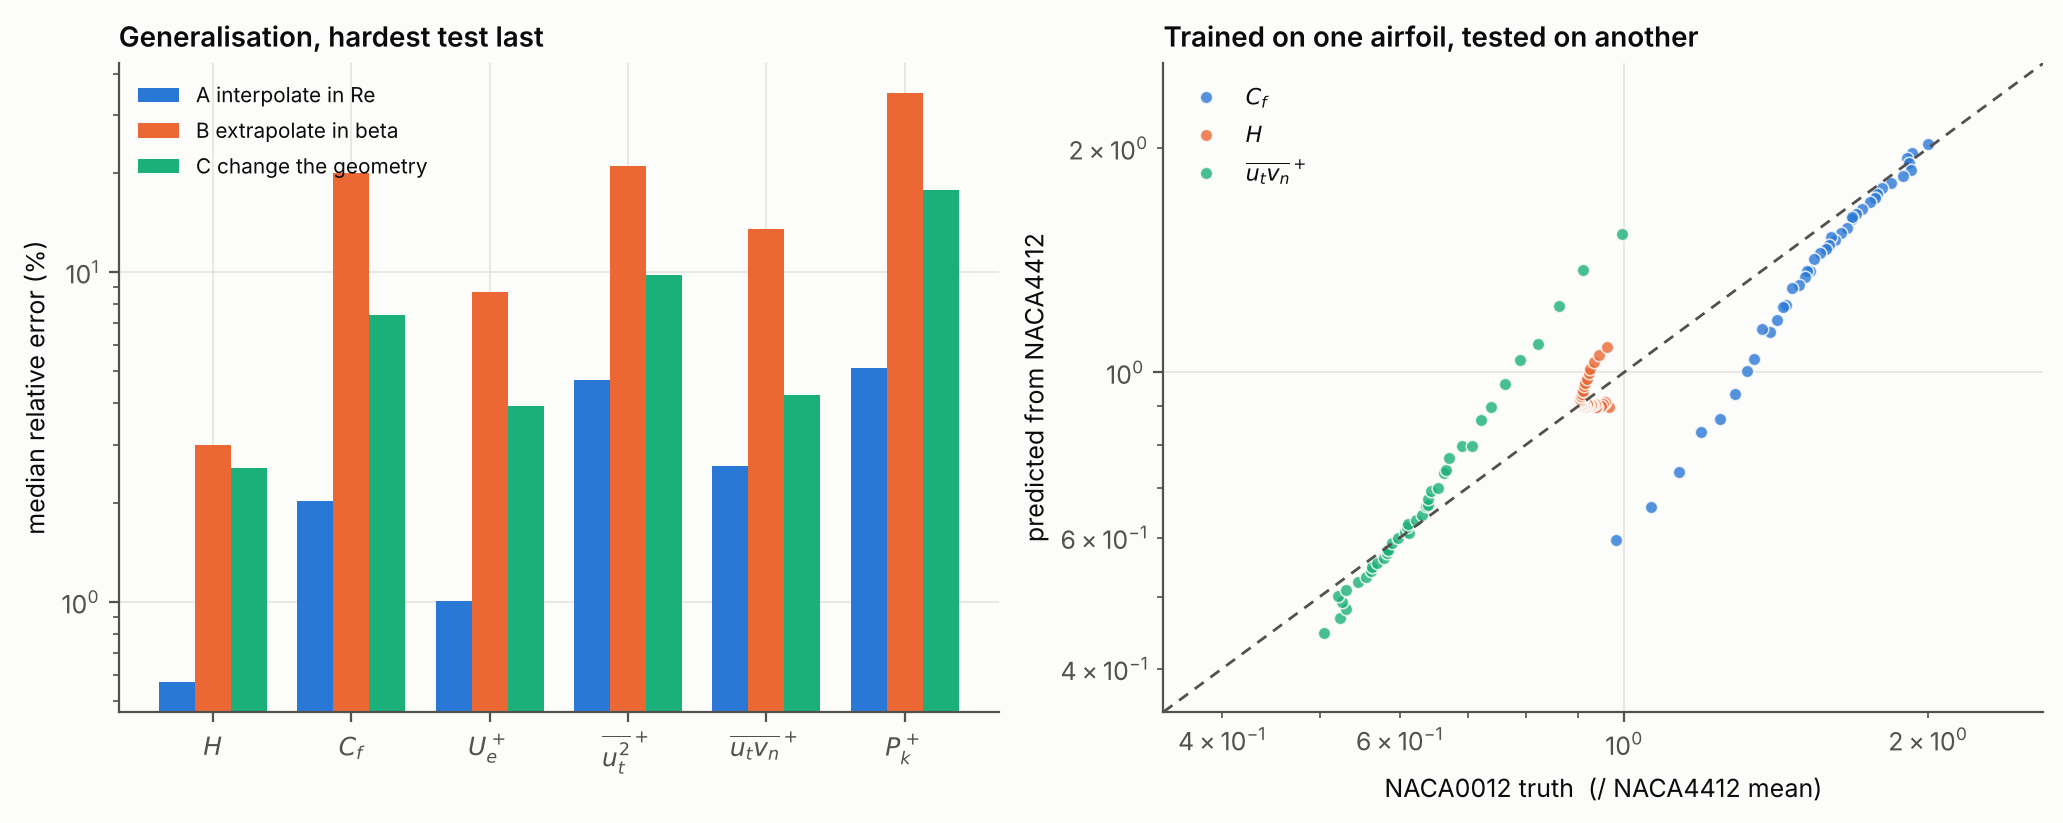
\includegraphics[width=\textwidth]{figures/fig_generalisation.png}
  \caption{\textbf{Left:} median relative error for the three tests.
  \textbf{Right:} the cross-geometry test, fitted on the NACA4412 at
  $5^\circ$ and evaluated on the NACA0012 at $0^\circ$, normalised by the
  training geometric mean so that three quantities share one pair of axes.}
  \label{fig:general}
\end{figure}

Table~\ref{tab:general} reports three tests of increasing severity.
Interpolating in Reynolds number is easy ($0.6$--$5.1\%$). Extrapolating
twenty-fold in $\beta$---trained on $x/c \le 0.70$ where
$\beta \le 2.5$, evaluated where $\beta$ reaches $49$---costs $20$--$35\%$
on $C_f$, $\overline{u_t^2}^+$ and $P_k^+$; the law should be used within its
calibration range. The cross-geometry test is the demanding one: fitted on a
cambered section at $5^\circ$ and applied unchanged to a \emph{symmetric}
section at $0^\circ$ whose pressure gradient reaches only $\beta = 3.3$, it
returns $2.5$--$9.8\%$ median error on five of six quantities.

A fourth test is impossible, and the reason is itself a result: the pressure
side is a favourable pressure gradient with $\beta < 0$ at $88$--$95\%$ of
stations in the window, and $\beta^{a_1}$ is not real there.
Equation~\eqref{eq:law} is an adverse-pressure-gradient law and does not
continue through $\beta = 0$; extending it would require a different form,
not a refit.

\begin{table}[t]
  \centering
  \small
  \caption{Median relative error (\%) for the three generalisation tests.}
  \label{tab:general}
  \begin{tabular}{lccc}
    \toprule
    target & A: hold out $\Rec=4\times10^5$ & B: extrapolate $\beta$ &
    C: NACA4412 $\to$ NACA0012 \\
    \midrule
    $H$                   & 0.57 &  2.99 &  2.54 \\
    $C_f$                 & 2.03 & 19.96 &  7.42 \\
    $U_e^+$               & 1.01 &  8.70 &  3.93 \\
    $\overline{u_t^2}^+$  & 4.72 & 20.96 &  9.81 \\
    $\overline{u_tv_n}^+$ & 2.59 & 13.54 &  4.24 \\
    $P_k^+$               & 5.11 & 34.98 & 17.72 \\
    \bottomrule
  \end{tabular}
\end{table}

\subsection{Is the three-term law the right complexity?}

We searched exhaustively over all 255 expressions of up to four terms drawn
from a nine-term library---powers of the three variables, their pairwise
products in log space, and quadratic curvature---at four memory lengths.
Exhaustive rather than genetic search removes the seed, population size and
stopping rule that would otherwise require justification, and is optimal
within the space considered.

Two findings. First, \textbf{the interaction $\log\beta \cdot
\log(\bbar/\beta)$ is selected for all six targets}, out of nine candidate
terms in six independent selections. Its presence means the exponent on
$\beta$ depends on how far the upstream history departs from the local
value: history and local pressure gradient \emph{multiply} rather than
acting as the separable factors that Equation~\eqref{eq:law} assumes. The
next most frequent terms are $\log^2\beta$ ($5/6$, curvature in $\beta$) and
$\log\beta\cdot\log\Ret$ ($4/6$, a Reynolds-dependent exponent on $\beta$).

Second, and cautionary, \textbf{selection optimism is a factor of $4.4$
(median, range $3.2$--$5.9$)}. The leave-one-Reynolds-number-out error used
to choose among roughly a thousand candidates understates true held-out
error by that much. Evaluated honestly on the NACA0012, which took no part
in selection, the searched four-term expressions beat the three-term power
law on only four of six targets. The Pareto front also shows a clear elbow
at three terms: the first three buy an order of magnitude in accuracy, the
fourth buys little. We therefore retain Equation~\eqref{eq:law} as the
working law and report the interaction as the indicated direction for a
richer form, rather than adopting the searched expressions wholesale.

\section{Discussion}

The decomposition splits the original finding in two. For the wall and
integral quantities and for TKE production, Reynolds number accounts for
$65$--$73\%$ of the difference between cases, and the conclusion of
\citet{vinuesa2018} is supported. For the outer-region Reynolds stresses it
accounts for only $23$--$36\%$, and the majority of the measured trend is
residual pressure-gradient sensitivity rather than a Reynolds-number effect.
Since the outer region is where the two proposed energising mechanisms were
argued to differ, this is the part of the argument most in need of the
larger database.

That the fitted memory length is short, $\ell \approx 0.5\,\dnn$, and
similar for inner and outer quantities deserves comment, since Clauser's
long-memory observation might predict otherwise. We initially obtained an
order-of-magnitude separation between wall and outer quantities by scanning
$\ell$ against held-out error; it did not survive selecting $\ell$ inside
the training fold with a non-collinear parameterisation. We report the
corrected result. Note that a short kernel is not the same as a weak
history effect: removing the history term entirely degrades the fit by a
factor of $10$--$24$, and the effect it captures is of order the local
boundary-layer thickness, which itself grows by an order of magnitude along
the chord.

\paragraph{Limitations.} The analysis rests on three Reynolds numbers of a
single section plus one cross-geometry case, so case-level statistics are
weak and we report case-level rather than station-level generalisation
throughout. The law has no favourable-pressure-gradient limit. The memory
length is identifiable only to a factor of order $1.3$. And $\beta$ is taken
as distributed rather than recomputed, since the 50 stored stations
under-resolve the pressure gradient. The natural next step is the database
of \citet{mallor2024}, which spans three Reynolds numbers and four angles
of attack: varying incidence changes $\beta(x)$ while holding the geometry
fixed, which is precisely the lever needed to separate history from local
magnitude with more than one pressure-gradient history per geometry.

\section{Conclusions}

\begin{enumerate}
  \item The matched-$\beta$ premise underlying the Reynolds-number
        comparison in \citet{vinuesa2018} holds only to tens of percent, and
        the residual is monotone in Reynolds number, so it is confounded
        with the effect being measured.
  \item A three-term power law with a fitted memory length predicts a
        held-out Reynolds number to $1.2$--$9.2\%$ and, being linear in
        logarithms, splits the difference between cases exactly.
  \item For the outer-region Reynolds stresses, $64$--$77\%$ of the apparent
        Reynolds-number trend is attributable to the residual $\beta$
        mismatch; for wall and integral quantities and TKE production,
        Reynolds number dominates.
  \item The law transfers from a cambered section at $5^\circ$ to a
        symmetric section at $0^\circ$ with $2.5$--$9.8\%$ median error on
        five of six quantities, but does not extrapolate far in $\beta$ and
        has no favourable-gradient limit.
  \item An exhaustive symbolic search selects the interaction between local
        $\beta$ and the memory ratio for every target, indicating that
        history and local pressure gradient multiply rather than acting
        separably.
\end{enumerate}

\section*{Data and code availability}

The WING database is the property of its authors; the download links
currently published are not operational, and the files used here were
supplied on request. All analysis code, the reproduction of
\citet{vinuesa2018}, and the scripts generating every figure and table in
this paper are available at \texttt{<repository URL>}, together with a
documented audit of the database.

\section*{Acknowledgements}

We thank R.\ Vinuesa for providing the database.

\begin{thebibliography}{9}
\small

\bibitem[Bobke et al.(2017)]{bobke2017}
A.~Bobke, R.~Vinuesa, R.~Örlü and P.~Schlatter.
History effects and near equilibrium in adverse-pressure-gradient turbulent
boundary layers.
\emph{J.\ Fluid Mech.}, 820:667--692, 2017.

\bibitem[Clauser(1956)]{clauser1956}
F.~H. Clauser.
The turbulent boundary layer.
\emph{Adv.\ Appl.\ Mech.}, 4:1--51, 1956.

\bibitem[Mallor et al.(2024)]{mallor2024}
F.~Mallor, R.~Vinuesa, R.~Örlü and P.~Schlatter.
High-fidelity simulations of the flow around a NACA 4412 wing section at high
angles of attack.
\emph{Int.\ J.\ Heat Fluid Flow}, 110:109590, 2024.

\bibitem[Pinkerton(1938)]{pinkerton1938}
R.~M. Pinkerton.
The variation with Reynolds number of pressure distribution over an airfoil
section.
\emph{NACA Report} 613, 1938.

\bibitem[Schlatter and Örlü(2010)]{schlatter2010}
P.~Schlatter and R.~Örlü.
Assessment of direct numerical simulation data of turbulent boundary layers.
\emph{J.\ Fluid Mech.}, 659:116--126, 2010.

\bibitem[Tanarro et al.(2020)]{tanarro2020}
A.~Tanarro, R.~Vinuesa and P.~Schlatter.
Effect of adverse pressure gradients on turbulent wing boundary layers.
\emph{J.\ Fluid Mech.}, 883:A8, 2020.

\bibitem[Vinuesa et al.(2016)]{vinuesa2016}
R.~Vinuesa, A.~Bobke, R.~Örlü and P.~Schlatter.
On determining characteristic length scales in pressure-gradient turbulent
boundary layers.
\emph{Phys.\ Fluids}, 28:055101, 2016.

\bibitem[Vinuesa et al.(2018)]{vinuesa2018}
R.~Vinuesa, P.~S. Negi, M.~Atzori, A.~Hanifi, D.~S. Henningson and
P.~Schlatter.
Turbulent boundary layers around wing sections up to
$\mathrm{Re}_c = 1{,}000{,}000$.
\emph{Int.\ J.\ Heat Fluid Flow}, 72:86--99, 2018.

\end{thebibliography}

\end{document}
